\section{Оборудование и инструментальные погрешности}

Уравновешенный гироскоп закреплён в кольцах карданова подвеса. Наружное кольцо А
свободно поворачивается вокруг вертикальной оси {\itshape аа}. Внутреннее кольцо
Б связано с кольцом А осью {\itshape бб}. В кольце Б укреплён гироскоп, ось вращения
которого {\itshape вв} перпендикулярна к оси {\itshape бб}. Центр масс гироскопа находится
на пересечении осей и покоится при вращении.

\begin{figure}
    \centering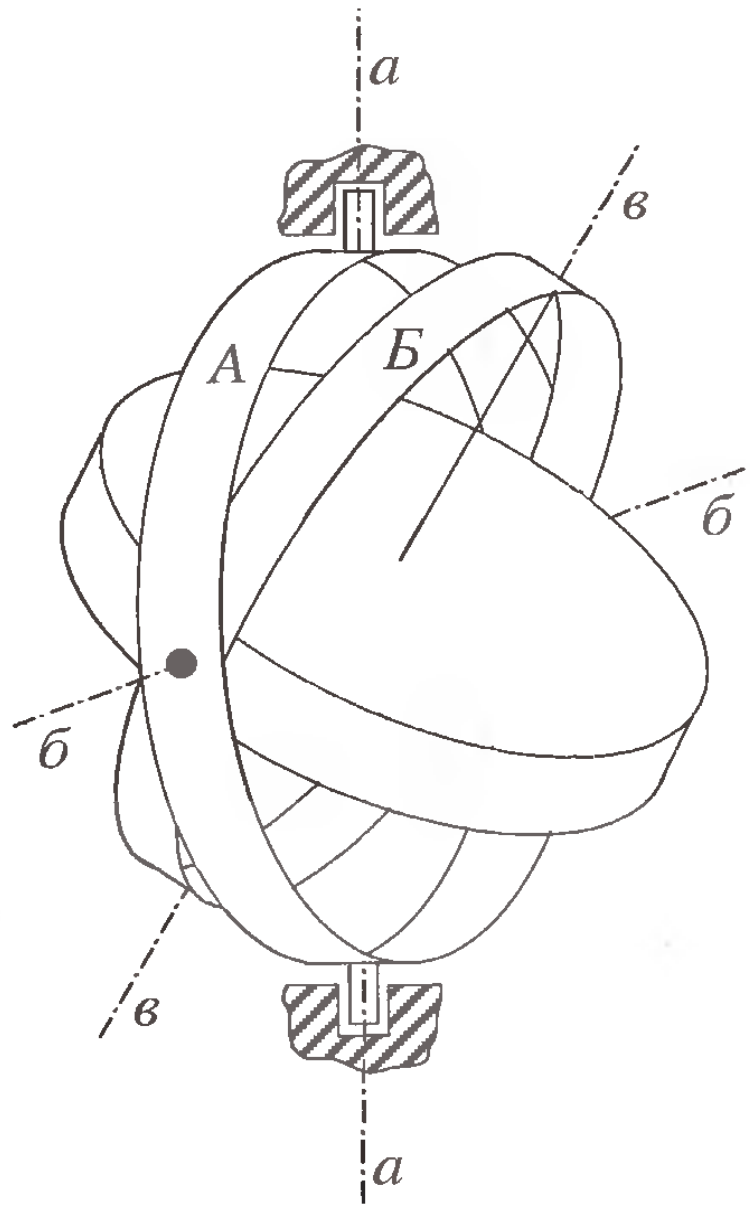
\includegraphics[width=0.5\linewidth]{img/hyr.png}
\end{figure}

\begin{figure}
    \centering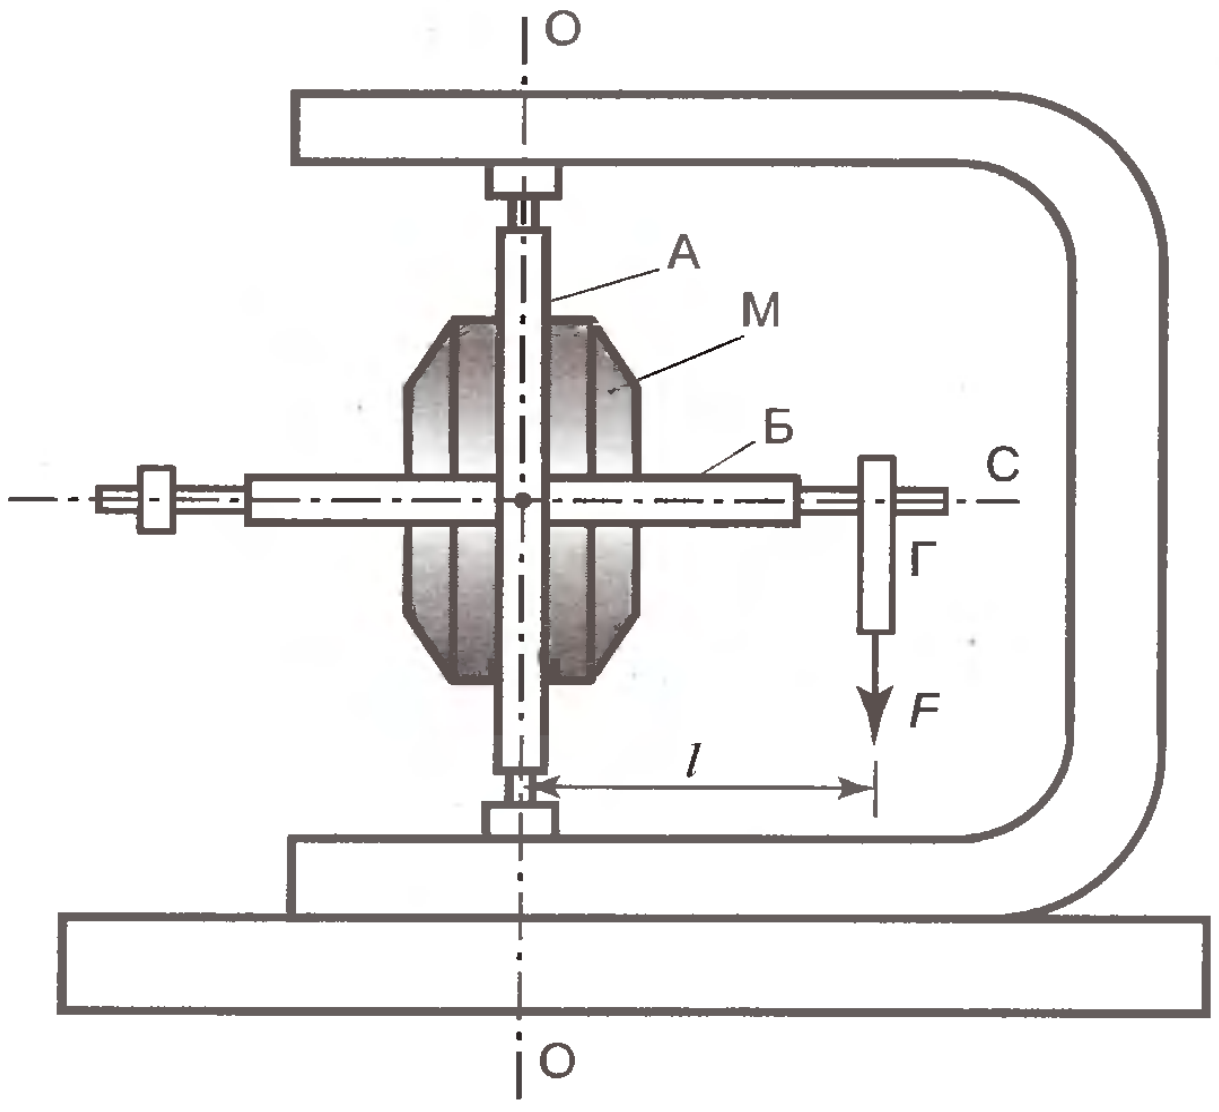
\includegraphics[width=0.5\linewidth]{img/hyr2.png}
\end{figure}

Ротор гироскопа~--- ротор высокооборотного электромотора М. Его кожух скреплён с кольцом Б.
Оно может вращаться в кольце А вокруг оси {\itshape бб}, которое вращается в оси {\itshape аа}.

Рычаг С направлен по оси симметрии ротора. На него подвешивают грузы Г.

Электродвигатель компенсирует силы трения и момент импульса гироскопа не меняется по модулю.
Из-за трения в осях ось гироскопа будет опускаться в направлении действия груза.

Для исследования зависимости скорости прецессии от момента силы к рычагу подвешиваются
грузы. Скорость прецессии определяется по числу оборотов рычага и времени, которое на это
ушло. В начале опыта рычаг надо поднять на $5$~--$6$ градусов, закончить, когда он на такой
же угол опустится вниз.

Момент иннерции ротора измеряется по крутильным колебаниям на проволоке. Период его
колебаний связан с периодом тела известного момента иннерции:
\[
    I_0=I\frac{T_0^2}{T^2}
\]

Угловая скорость вращения исследуется по частоте генерируемой ЭДС в обмотке.